\subsection{内存}

内存控制器(RamControllor),用来提供所有存储设备与外设接口的控制信号,是CPU与外部存储单元的唯一交互接口。为了避免取指与访存的结构冲突,我们设计了两个RAM控制器:RAM2用于映射指令内存,RAM1用于映射数据内存、屏幕显存和FIFO(对于它们的介绍详见外设部分)。对CPU来说,所有的存储单元均采用统一编码的地址(称\textbf{逻辑地址})进行访问,其与物理地址或外部设备的映射关系如\tref{table:mem_addr}所示。地址线为16位。

\begin{center}
    \tcaption{内存地址空间映射}\label{table:mem_addr}
    \begin{longtable}{ll}
        \toprule
        逻辑地址 & 映射到的物理地址或设备 \\
        \midrule
        0x0000 $\thicksim$ 0x7FFF & RAM2 0x0000 $\thicksim$ 0x7FFF \\
        0x8000 $\thicksim$ 0xBEFF & RAM1 0x0000 $\thicksim$ 0x3EFF \\
        0xBF00 & 串口控制信号 \\
        0xBF01 & 串口数据(低8位有效) \\
        0xBF02 & 串口2控制信号(未使用) \\
        0xBF03 & 串口2数据(未使用) \\
        0xBF04 & FIFO1读取数据 \\
        0xBF05 & FIFO2控制信号(队列是否为空) \\
        0xBF06 & FIFO2读取数据 \\
        0xBF07 & FIFO2写入数据 \\
        0xBF08 & 显存写入地址高16位 \\
        0xBF09 & 高3位为显存写入地址低3位,最低位为数据位 \\
        0xBF0A $\thicksim$ 0xBF0F & 保留 \\
        0xBF10 $\thicksim$ 0xFFFF & RAM1 0x3F10 $\thicksim$ 0x7FFF \\
        \bottomrule
    \end{longtable}
\end{center}

各设备访问时序如下:

% http://wavedrom.com/editor.html
% {signal: [
%   {name: 'data', wave: 'x2..|z.x2..', data: ['write data', 'read data']},
%   {name: 'addr', wave: 'x2..|x2...x', data: ['write addr', 'read addr']},
%   {name: 'OE', wave: '1...|0.....'},
%   {name: 'WE', wave: '1.01|......'},
%   {name: 'EN', wave: '0...|......'},
% ]}

\begin{center}
    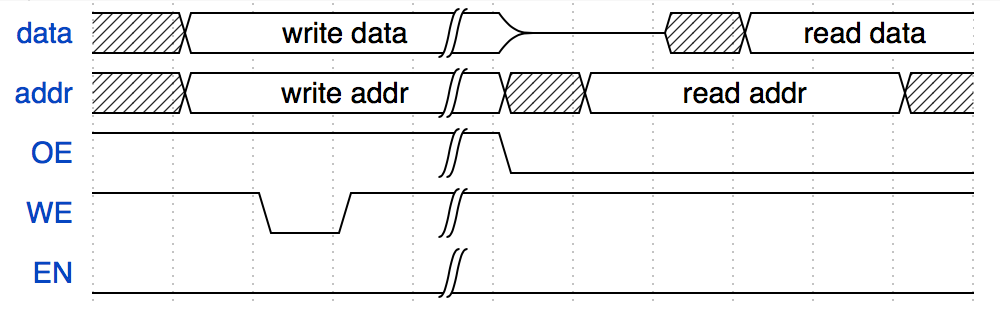
\includegraphics[width=11cm]{image/device/sram}
    \fcaption{SRAM访问时序}
\end{center}

% {signal: [
%   {name: 'data', wave: 'x2..|zx2.z', data: ['write data', 'read data']},
%   {name: 'wrn', wave: '101.|.....'},
%   {name: 'rdn', wave: '1...|.0..1'}
% ]}

\begin{center}
    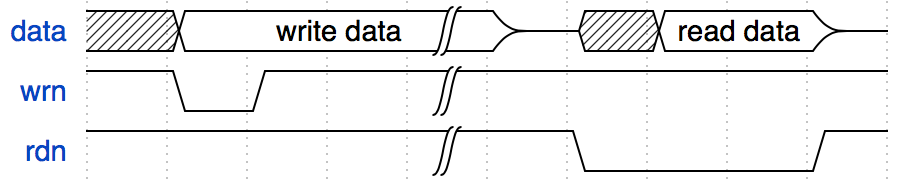
\includegraphics[width=11cm]{image/device/serial}
    \fcaption{串口访问时序}
\end{center}

% {signal: [
%   {name: 'clk', wave: '01|010'},
%   {name: 'data', wave: '2.|x..', data: ['write data']},
%   {name: 'addr', wave: '2.|2..', data: ['write addr', 'read addr']},
%   {name: 'dout', wave: 'x.|x2.', data: ['read data']},
%   {name: 'wr_en', wave: '1.|0..'},
%   {name: 'rd_en', wave: '0.|1..'}
% ]}

\begin{center}
    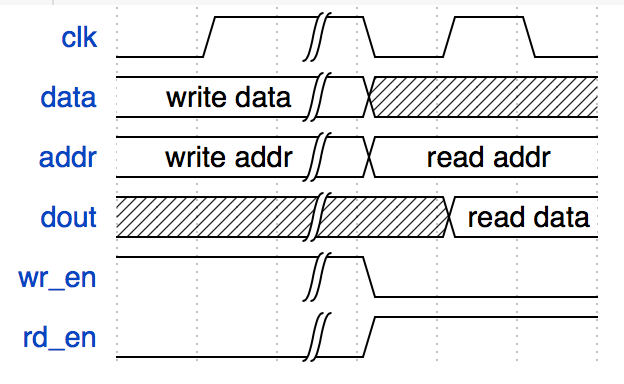
\includegraphics[width=8cm]{image/device/vga}
    \fcaption{显存访问时序(上升沿触发)}
\end{center}

% {signal: [
%   {name: 'clk', wave: '01|010'},
%   {name: 'data', wave: '2.|x..', data: ['write data']},
%   {name: 'dout', wave: 'x.|x2.', data: ['read data']},
%   {name: 'wr_en', wave: '1.|0..'},
%   {name: 'rd_en', wave: '0.|1..'}
% ]}

\begin{center}
    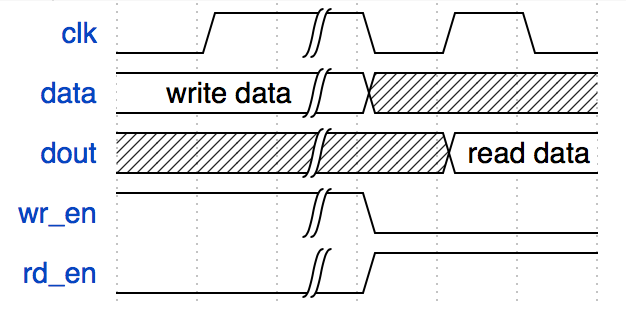
\includegraphics[width=8cm]{image/device/fifo}
    \fcaption{FIFO访问时序(上升沿触发)}
\end{center}

控制器采用两倍于CPU主频的时钟下降沿触发,分别在两个状态$S_1$与$S_2$之前跳转。对于不同访存的需求,各状态更新的控制信号如\tref{table:mem_signals}所示。初始状态下,OE, WE, rdn, wrn均为1,使能均关闭。

\begin{center}
    \tcaption{内存控制器状态转换}\label{table:mem_signals}
    \begin{longtable}{p{0.15\columnwidth}p{0.05\columnwidth}p{0.4\columnwidth}p{0.4\columnwidth}}
        \toprule
        设备 & 读/写 & $S_1$ & $S_2$ \\
        \midrule
        SRAM & 读 & OE置0,WE置1,数据线置高阻,地址线置待读取地址 & 锁存读出的数据 \\
        SRAM & 写 & OE置1,WE置1,数据线置待写入数据,地址线置待写入地址 & WE置0 \\
        串口控制 & 读 & - & 锁存输出的控制信号 \\
        串口数据 & 读 & rdn置0,wrn置1,数据线置高阻 & 锁存读出的数据,rdn置1 \\
        % 串口数据 & 写 & - & rdn置0,wrn置0,数据线置待写入数据 & wrn置0 \\
        显存地址 & 写 & 锁存地址高16位 & - \\
        显存数据 & 写 & 准备地址和数据,开启写使能,写时钟置0 & 写时钟置1 \\
        FIFO测试 & 读 & - & 锁存输出的控制信号 \\
        FIFO & 读 & 开启读使能 & 锁存读出的数据,关闭读使能 \\
        FIFO & 写 & 准备地址和数据,开启写使能,写时钟置0 & 写时钟置1 \\
        \bottomrule
    \end{longtable}
\end{center}

其中,显存与FIFO采取异步写,同步读的方式。FIFO的读时钟与控制器同频率,但是采用上升沿触发。该部件的控制信号如\tref{table:memory_ctl}所示。

\begin{center}
    \tcaption{内存控制器信号}\label{table:memory_ctl}
    \begin{longtable}{p{0.3\columnwidth}p{0.7\columnwidth}}
        \toprule
        信号 & 信号描述 \\
        clk & 控制器时钟。 \\
        rst & 异步清空信号,由外部控制开关接入。 \\
        in\_pc\_addr & 指令地址。 \\
        in\_ram\_addr & 访存地址。 \\
        in\_data & 写入数据。 \\
        in\_rd & 读使能。 \\
        in\_wr & 写使能。 \\
        out\_data & 读出数据。 \\
        out\_pc\_ins & 取出指令。 \\
        slow\_clk & CPU时钟,用于初始状态同步。 \\
        ram2\_oe & RAM2 OE控制输出。 \\
        ram2\_we & RAM2 WE控制输出。 \\
        ram2\_en & RAM2 EN控制输出。 \\
        ram2\_addr & RAM2 地址线输出。 \\
        ram2\_data & RAM2 数据总线。 \\
        ram1\_oe & RAM1 OE控制输出。 \\
        ram1\_we & RAM1 WE控制输出。 \\
        ram1\_en & RAM1 EN控制输出。 \\
        ram1\_addr & RAM1 地址线输出。 \\
        ram1\_data & RAM1 数据总线。 \\
        serial\_rdn & 串口rdn控制。 \\
        serial\_wrn & 串口wrn控制。 \\
        serial\_data\_ready & 串口data\_ready输入。 \\
        serial\_tbre & 串口tbre输入。 \\
        serial\_tsre & 串口tsre输入。 \\
        vga\_data & 显存写入数据。 \\
        vga\_addr & 显存写入地址。 \\
        vga\_data\_clk & 显存写时钟。 \\
        fifo1\_rd\_en & FIFO1读使能。 \\
        fifo1\_data & FIFO1读出数据。 \\
        fifo2\_rd\_en & FIFO2读使能。 \\
        fifo2\_wr\_clk & FIFO2写时钟。 \\
        fifo2\_data\_in & FIFO2写入数据。 \\
        fifo2\_data\_out & FIFO2读出数据。 \\
        fifo2\_is\_empty & FIFO2控制输入(是否为空)。 \\
        \midrule
        \bottomrule
    \end{longtable}
\end{center}
